\documentclass[12pt]{article}
\usepackage{graphicx} % Required for inserting images
\graphicspath{images/} % Direct to "images" folder
\usepackage{subcaption} 
\usepackage{caption}      
\usepackage{float} 
\usepackage{conveniences}
\usepackage{geometry}
\usepackage{ragged2e}
\usepackage{amssymb}
\usepackage{titlesec}
\usepackage{fancyhdr}
\usepackage{xcolor}
\usepackage[titles]{tocloft}  % Allows customization of ToC layout
\usepackage{etoolbox}
\usepackage{comment}
\usepackage{hyperref}

\titleformat{\section}
    {\centering\fontS{18}\bfseries} %Centered, Font 18, Bold
    {\thesection} %No numbering
    {0.5em} %No extra space
    {} %No extra formatting
    [\vspace{20pt}\titlerule\vspace{10pt}]

\begin{document}
\begin{center}
    
\includegraphics[width=\linewidth]{NTU_Logo.png}
    \\[1cm]
    \fontS{20}
    \underline{\textbf{SC4020 Data Analytics and Mining}}
    \\[1.5em]
    \fontS{14}
    Academic Year 2025/2026
    \\[1em]
    Semester 1
    \\[2em]
    Group 18
    \\[5em]
    \textbf{
        LUNBERRY NOAH IWATA (N2503869H) \\[1em]
        PIKERINGA ANTONINA DAILA (N2504101A) \\[1em]
        RAHLFS FREDERIC MAURITZ (N2504096K) \\[1em]
        SARAH EMILY ONG XIN WEI (U2440124G) \\[1em]
        }
\end{center}
\pagebreak

\justifying

\pagestyle{fancy}
\fancyhf{}  % Clear default header/footer
\fancyhead[R]{\textcolor{gray}{\nouppercase{\leftmark}}}   % Left header shows current section title
\fancyfoot[C]{\thepage}  % Footer center shows page number

\pagenumbering{roman}

\section*{Abstract}
\markboth{Abstract}{} 
\addcontentsline{toc}{section}{Abstract} 

There is nothing wrong with second place.
Your best effort is all that anyone's asking for.
And if you give your best and you come in second, you come in third, you come in last, it's not about winning or losing.
It's about giving it everything you've got.
Now, Sam has built a monument to devilry and chaos.
I deserve second place, I came in second.
The only crime that's been committed here is that Oscar and Ally deserve first.
We should be applauding them for getting more points.
But in this sick rodeo, this bizarre \textit{fucked up} clown festival that Sam's put together, we're here celebrating what I can only describe as the sickness at the core of America.
And I'm gonna get him, I'm gonna get Sam.

\pagebreak
\renewcommand{\cftdotsep}{0.5}
\renewcommand{\cftsecleader}{\cftdotfill{\cftdotsep}}
\renewcommand{\contentsname}{Table of Contents}  % Set ToC title text
\setlength{\cftbeforesecskip}{10pt}   % Space before sections
\setlength{\cftbeforesubsecskip}{10pt} % Space before subsections
\setlength{\cftbeforesubsubsecskip}{10pt} % Space before subsections
\renewcommand{\cftsecpresnum}{Chapter~} % Adds "Chapter" before section number
\renewcommand{\cftsecaftersnum}{\quad} 
\setlength{\cftsecnumwidth}{6.1em}   %hardcoded in, will die if you have double digit chapters
%\renewcommand{\numberline}[1]{Chapter #1\quad} %old code, works as well but add Chapter to the subsections too which is L
\tableofcontents

\pagebreak
\pagenumbering{arabic}
\section{Introduction}

\subsection{Motivation for Research}

This research was motivated by the 4AUs it carries (not worth it)

\subsection{Objectives}

\subsection{Scope of Work}

\subsection{Organisation of Report}

\pagebreak
\section{Methods}
In order to accurately assess the capability of two different graph networks, two diverse datasets were chosen. The two models were trained on each and evaluated.

\subsection{Datasets}
The two datasets used in this study were the NASA Turbofan Jet Engine Degradation dataset (C-MAPSS) and the UCI Wisconsin Breast Cancer dataset. These were selected to reflect two distinct real-world problems. Prognostics of mechanical systems and medical diagnosis. This ensured diversity in the training data while reducing domain-specific bias.

The Wisconsin Breast Cancer dataset consists of 32 columns. Two columns correspond to identifiers and diagnosis labels, respectively.
The remaining 30 represent measurable tumor characteristics (e.g., radius, texture, area, smoothness, compactness, concavity, etc.). The target variable is the classification of the tumor as benign or malignant. Before training, all numerical features were normalized to zero mean and unit variance to ensure convergence during training. The dataset was split into training and test sets using an 80/20 ratio.


The NASA C-MAPSS turbofan jet engine degradation dataset provides multivariate time-series data simulating total life scenarios of jet engines. Each engine instance is characterized by 26 columns: one engine identifier, one time cycle index, three operational condition variables, and 21 sensor measurements. The target variable is the Remaining Useful Life (RUL), defined as the number of cycles left until engine failure.
The dataset was provided with separate training and validation partitions: 100 engines for training and 100 engines for validation. For consistency, sensor features were normalized across engines.


The two datasets differ fundamentally, both in data modality (tabular biomedical features vs. multivariate time-series sensor data) and in target type (classification vs. regression). This diversity was intentional, aiming to assess the generalizability of the evaluated models across domains.


\subsection{Models}
Two graph networks with different layers were used.
For the breast cancer dataset, nodes corresponded to patient samples, while the edges were chosen according to a k-NN graph. Node features corresponded to the 30 tumor attributes, and the output task was binary classification.
For the turbofan dataset, nodes represented sensor states and operational conditions. Edges were defined through feature correlations. The GCN then predicted the Remaining Useful Life (RUL)
as a regression task.

\subsubsection{Graph Convolutional Network (GCN)}
The Graph Convolutional Network (GCN) serves as a baseline model for learning from graph-structured data. A GCN updates node representations by aggregating feature information from neighboring nodes.
The GCN architecture consisted of 2 convolutional layers with a  RELU activation function, and dropout for regularization.

\subsubsection{Graph Attention Network (GAT)}
The Graph Attention Network (GAT) extends the GCN by introducing an attention mechanism over neighboring nodes. Instead of averaging features uniformly, GAT learns attention coefficients that weight the contribution of each neighbor during aggregation. This allows the model to focus on the most informative relationships within the graph, which, especially in datasets with high assumed covariance, can lead to significantly improved results.
The GAT architecture consisted of 2 attention layers with 8 attention heads, followed by RELU. Again, dropout was used for regularization.

\subsection{Training, Inference, and Evaluation}
Both models were trained for 300 epochs on the NASA dataset, using MSE error due to the regressional nature of the target variable.

For the breast cancer dataset cross-entropy loss was employed due to the classification nature of the target, with 100 epochs.
The trained models were then used for inference on the validation dataset and compared to the reference. For the breast cancer dataset, an F1 score was used for evaluation, while for the NASA dataset, the MSE is used to compare the performance.
\pagebreak

\section{Results} \label{sec_results}
\autoref{sec_results} will present the results of the models' predictions. \autoref{sec_analysis} will analyse and draw conclusions from these results.

\subsection{Breast cancer dataset}
\subsubsection{GAT model}

For the breast cancer dataset, I used a Graph Attention Network (GAT). Each patient was a node in the graph, and edges were made using the ten closest patients based on how similar their features were. The graph ended up with 569 nodes and 8,326 edges. I split it into 455 for training and 114 for testing.

The GAT had two attention layers with eight heads each. I trained it for 100 rounds using cross-entropy loss. The loss started around 0.23 and went down to about 0.11 by the end, which means the model was learning steady.

\begin{table}[H]
\centering
\caption{GAT results on breast cancer dataset}
\begin{tabular}{|l|c|}
\hline
\textbf{Metric} & \textbf{Score} \\
\hline
Accuracy  & 0.9561 \\
Precision & 0.9512 \\
Recall    & 0.9286 \\
F1-Score  & 0.9398 \\
ROC-AUC   & 0.9944 \\
\hline
\end{tabular}
\end{table}

The GAT model did pretty well. It could tell benign and malignant tumors apart most of the time. The recall was a bit lower than the precision, so it missed a few malignant cases, but not many. The ROC-AUC score shows it still handles both classes very well. The attention part probably helped by letting the model focus on the more important neighbor nodes instead of averaging everyone the same way.

\subsubsection{GCN model}

I also report the Graph Convolutional Network (GCN) for the same data. Each patient is a node. We make edges with a $k$-NN graph (here $k=8$ like the code). Node features are the 30 tumor stats. The task is the same binary label.

We trained for 200 epochs with cross-entropy. Loss went down over time (e.g., 0.11 at epoch 20, then ~0.07 by the end). The final test accuracy was $0.9561$.

\begin{table}[H]
\centering
\caption{GCN results on breast cancer dataset}
\begin{tabular}{|l|c|}
\hline
\textbf{Metric} & \textbf{Score} \\
\hline
Accuracy  & 0.9561 \\
Precision & --- \\
Recall    & --- \\
F1-Score  & --- \\
ROC-AUC   & --- \\
\hline
\end{tabular}
\end{table}

\subsection{NASA turbofan jet engine dataset} 

\subsubsection{MSE error}

\autoref{table_NASA_MSE} shows the MSE error of both the GCN and GAT models. The GCN and GAT models have approximately the same MSE error, differing by less than 0.1\%. 

\begin{table}[H]
\centering
\caption{NASA turbofan jet engine: GCN vs GAT comparison}
\begin{tabular}{|l|c|}
\hline
\textbf{Model} & \textbf{MSE error}\\
\hline
GCN & 1365.4297  \\
GAT & 1363.8159  \\
\hline
\end{tabular}
\label{table_NASA_MSE}
\end{table}

\subsubsection{GCN model plots}
The results of the GCN model on the NASA turbofan jet engine dataset vary: \autoref{fig_NASA_GCN_eng6} is an example of a good fit of data, with the predictions well aligned with the true values. Other than some small spikes in the data, the overall downward slope is roughly accurate. \autoref{fig_NASA_GCN_eng4} shows an example of slight bias, with the slope of the predicted values being mostly correct but all predicted values being shifted upwards of the actual values by the same amount. \autoref{fig_NASA_GCN_eng2} and \autoref{fig_NASA_GCN_eng3} show moderate and high levels of bias respectively. Again, the slope of the predicted values is mostly accurate, but all predicted values are vertically shifted from true values. Interestingly, the example with the most bias (\autoref{fig_NASA_GCN_eng3}) has a much smoother slope than the examples with less bias. 

\begin{figure}[H]
    \centering

    \begin{subcaptionbox}{Good fit\label{fig_NASA_GCN_eng6}}[0.45\textwidth]
        {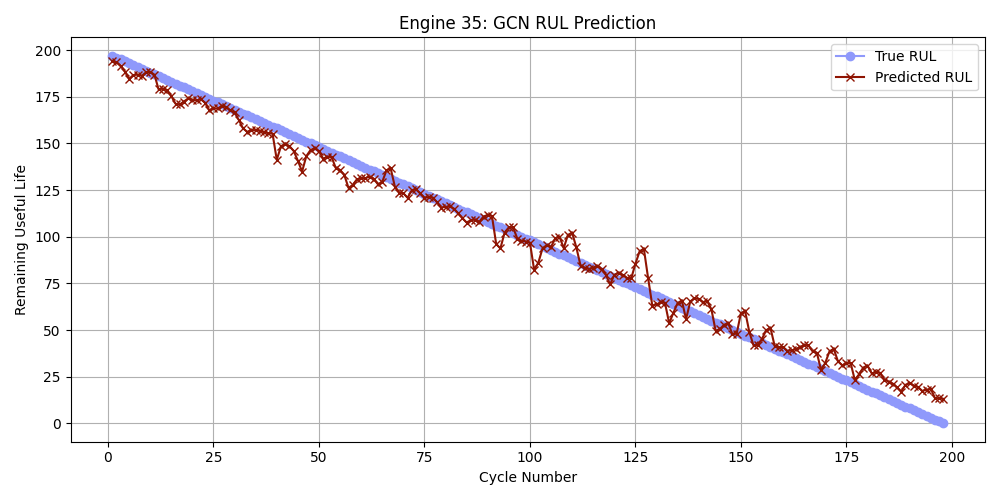
\includegraphics[width=\linewidth]{figures/NASA/NASA_GCN_eng6.png}}
    \end{subcaptionbox}
    \hfill
    \begin{subcaptionbox}{Slight bias\label{fig_NASA_GCN_eng4}}[0.45\textwidth]
        {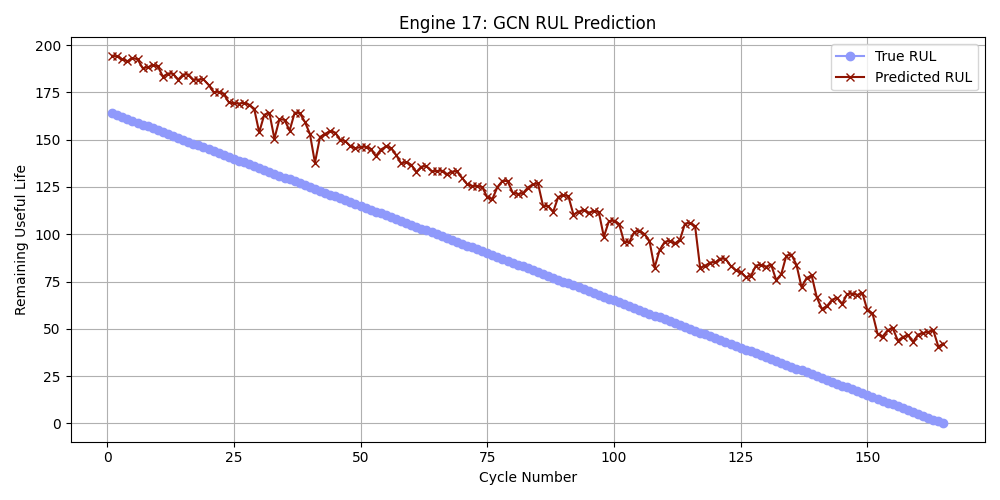
\includegraphics[width=\linewidth]{figures/NASA/NASA_GCN_eng4.png}}
    \end{subcaptionbox}

    \vspace{0.5cm}

    \begin{subcaptionbox}{Moderate bias\label{fig_NASA_GCN_eng2}}[0.45\textwidth]
        {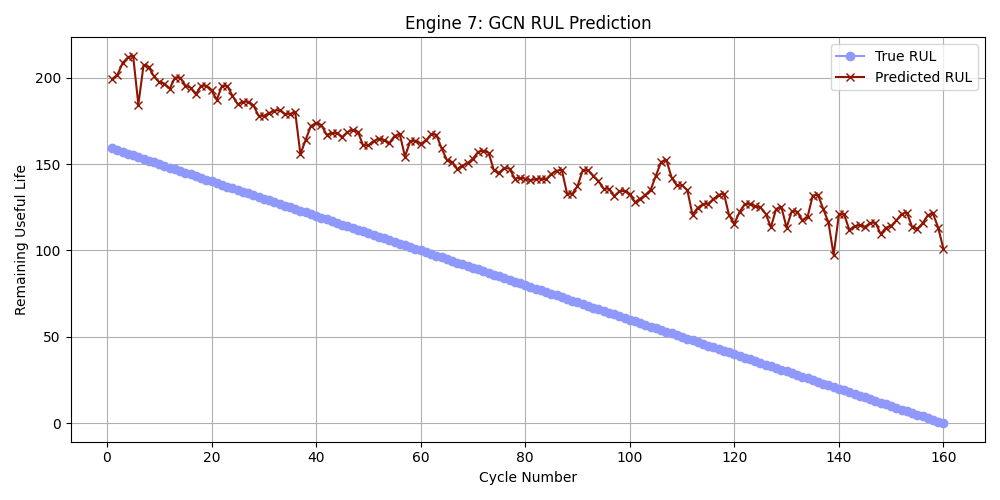
\includegraphics[width=\linewidth]{figures/NASA/NASA_GCN_eng2.png}}
    \end{subcaptionbox}
    \hfill
    \begin{subcaptionbox}{High bias\label{fig_NASA_GCN_eng3}}[0.45\textwidth]
        {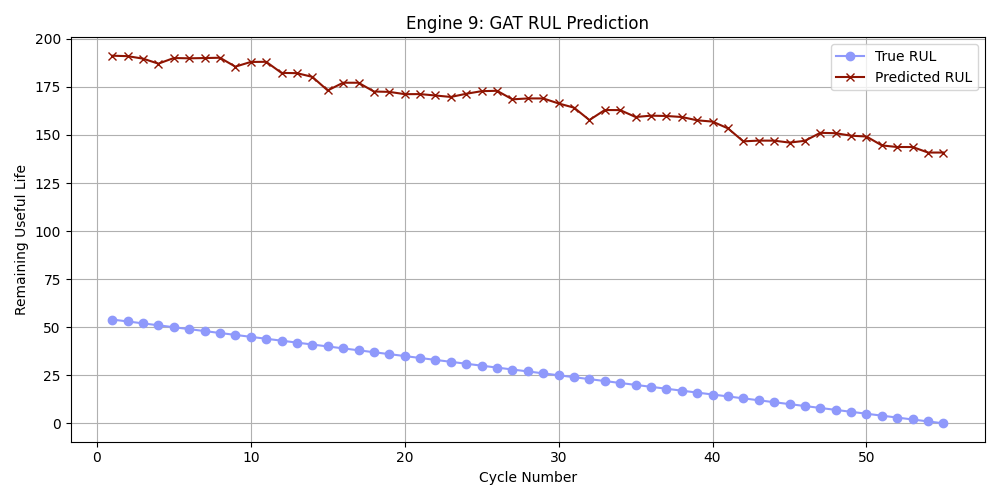
\includegraphics[width=\linewidth]{figures/NASA/NASA_GAT_eng3.png}}
    \end{subcaptionbox}

    \caption{GCN model on NASA data}
    \label{GCN_NASA_all}
\end{figure}


\subsubsection{GAT model plots}

The results of the GAT model on the NASA turbofan jet engine dataset follow a similar trend those of the GCN model. Instances of good fits (\autoref{fig_NASA_GAT_eng6}), slight bias (\autoref{fig_NASA_GAT_eng4}), moderate bias (\autoref{fig_NASA_GAT_eng2}), and high bias (\autoref{fig_NASA_GAT_eng3}) can be found. The GAT model also has small spikes in the predicted values, but overall the slopes of the predicted values are accurate.


\begin{figure}[H]
    \centering

    \begin{subcaptionbox}{Good fit\label{fig_NASA_GAT_eng6}}[0.45\textwidth]
        {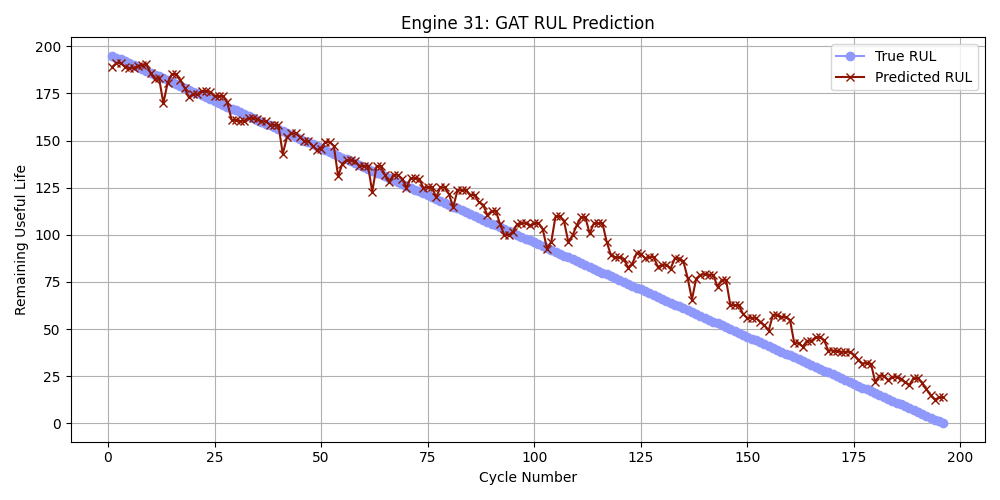
\includegraphics[width=\linewidth]{figures/NASA/NASA_GAT_eng7.png}}
    \end{subcaptionbox}
    \hfill
    \begin{subcaptionbox}{Slight bias\label{fig_NASA_GAT_eng4}}[0.45\textwidth]
        {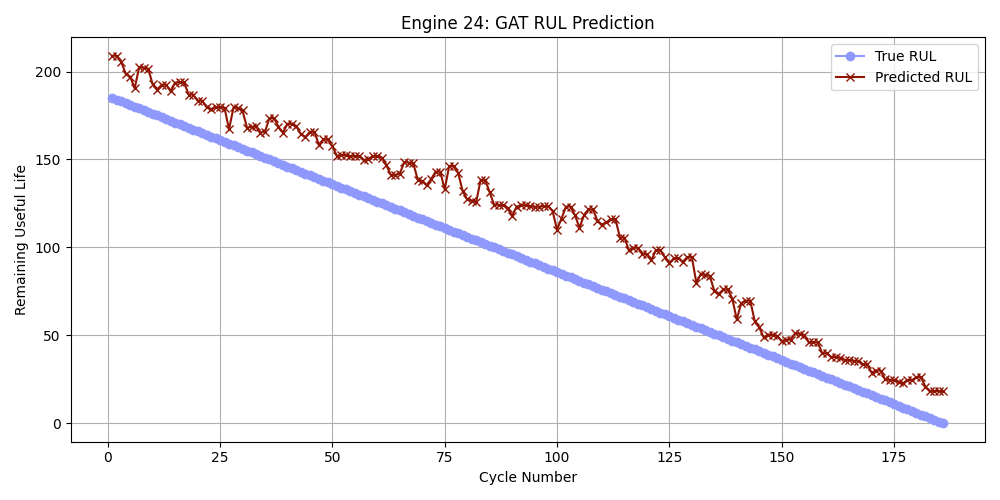
\includegraphics[width=\linewidth]{figures/NASA/NASA_GAT_eng6.png}}
    \end{subcaptionbox}

    \vspace{0.5cm}

    \begin{subcaptionbox}{Moderate bias\label{fig_NASA_GAT_eng2}}[0.45\textwidth]
        {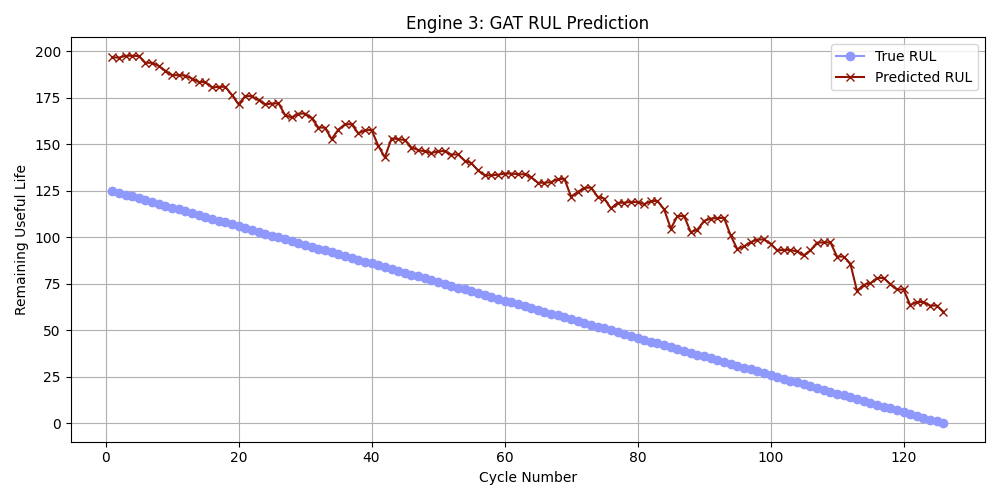
\includegraphics[width=\linewidth]{figures/NASA/NASA_GAT_eng1.png}}
    \end{subcaptionbox}
    \hfill
    \begin{subcaptionbox}{High bias\label{fig_NASA_GAT_eng3}}[0.45\textwidth]
        {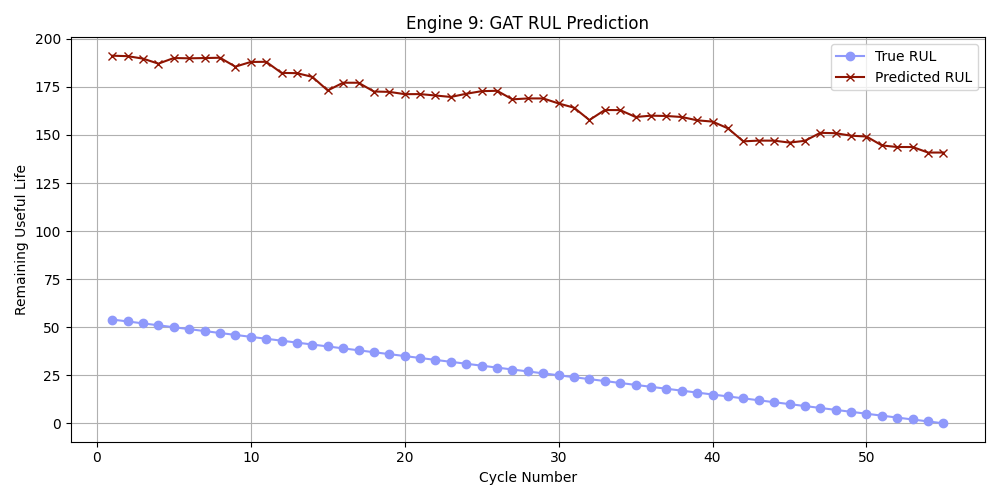
\includegraphics[width=\linewidth]{figures/NASA/NASA_GAT_eng3.png}}
    \end{subcaptionbox}

    \caption{GAT model on NASA data}
    \label{GAT_NASA_all}
\end{figure}


\pagebreak
\section{Analysis} \label{sec_analysis}

\subsection*{Breast cancer dataset: GAT vs GCN (short analysis)}

Both models hit the same test accuracy ($0.9561$). That tells me the dataset is clean and not too hard. The GAT shows a strong ROC-AUC ($0.9944$) and good F1 ($0.9398$), with recall $0.9286$. So it catches most malignant cases, while keeping precision high.

The main difference: GCN averages neighbors; GAT learns weights for each neighbor. On this data the gain is small but real in AUC. That fits our expect: attention helps when some neighbors matter more than others. If we align $k$ (Sarah used $k{=}8$, my GAT used $k{=}10$) we may see tiny shifts, but likely the same story.
\begin{table}[H]
\centering
\caption{Breast cancer: GAT vs GCN comparison}
\begin{tabular}{|l|c|c|c|c|c|}
\hline
\textbf{Model} & \textbf{Accuracy} & \textbf{Precision} & \textbf{Recall} & \textbf{F1} & \textbf{ROC-AUC} \\
\hline
GAT (ours) & 0.9561 & 0.9512 & 0.9286 & 0.9398 & 0.9944 \\
GCN (Sarah) & 0.9561 & --- & --- & --- & --- \\
\hline
\end{tabular}
\end{table}

\subsection{NASA turbofan jet engine dataset: GCN vs GAT}
The GCN and GAT models have similar MSE errors (see \autoref{table_NASA_MSE}), indicating similar performance. This can be confirmed by analysing plots of the predicted RUL values against the true RUL values, as shown in \autoref{GCN_NASA_all} and \autoref{GAT_NASA_all}. While both models have small oscillations throughout their predicted values, the models capture the general downward trend of the RUL data quite successfully. 

Varying levels of bias can be seen in the predictions. In an attempt to explain this bias, the RUL values were normalised. This is because the range of RUL values in the datasets was large, with some engines having RULs in the range of 50, while others - 200. The cycle numbers can also range from ranges of 60 to ranges of 200. This makes it difficult for the models to predict precise values across all engines. Predictions display the least bias for the engines having RULs in the range of 200, and the most bias for those with RULs in the range 50. Unfortunately, the normalisation attempts the did not fix the bias, hence further investigation is required to solve this issue.

\subsection{Comparison of GCN vs GAT across both datasets}

\pagebreak
\section{Conclusion}

\subsection{Heading}

\pagebreak
\section*{List of References}
\pagenumbering{arabic}
\renewcommand{\thepage}{R-\arabic{page}}
\markboth{List of References}{} 
\addcontentsline{toc}{section}{List of References}

\begin{comment}
    \pagebreak
    \section*{Appendix A - Heading}
    \pagenumbering{arabic}
    \markboth{Appendix A - Heading}{} 
    \renewcommand{\thepage}{A-\arabic{page}}
    \addcontentsline{toc}{section}{Appendix A - Heading}

    \pagebreak
    \section*{Appendix B - Heading}
    \pagenumbering{arabic}
    \markboth{Appendix B - Heading}{} 
    \renewcommand{\thepage}{B-\arabic{page}}
    \addcontentsline{toc}{section}{Appendix B - Heading}
\end{comment}

\end{document}
